%\documentclass{article}
%\usepackage[utf8x]{inputenc}
%\usepackage[T1]{fontenc}
%\usepackage[french]{babel}
%\usepackage{graphicx}
%\usepackage{vmargin}
%\usepackage{moreverb}
%\usepackage{tikz}
%\usepackage{algpseudocode}
%\usepackage{algorithm}
%%\usepackage{algorithmicx}
%\setmarginsrb{2cm}{2cm}{2cm}{2cm}{0cm}{0cm}{0cm}{0cm}
%
%\frenchbsetup{StandardLists=true}
%
%\title{Logique : Prise de notes - Groupe 23}
%\author{Bellenger Jordan \and Schmitz Loic \and Dethise Arnaud}
%\date{17 décembre 2014}
%
%\begin{document}
%
%\maketitle

\section{Structure du Web} %chapitre 13


\subsection{Mémoire associative - Hypertexte}

Liens hypertextes : chaque élément a des liens vers et depuis d'autres éléments. Un contenu hypertexte est un contenu auquel il est fait référence dans un document.

\vspace{0.5cm}
Deux exemples de contenus hypertextes :

$
\left. 
%\text{
\parbox{0.5\linewidth}{
\begin{itemize}
\item \textbf{Graphe de citations} \\
		Précurseur du web : nœuds indépendants, liens strictement vers le passé
\item \textbf{Encyclopédie} \\
		Les articles renvoient vers d'autres articles \\ (Wikipédia)
\end{itemize}
}%}
\hspace{0.5cm} \right\}
$ Réseaux d'informations




\begin{figure}[!h]
\centering
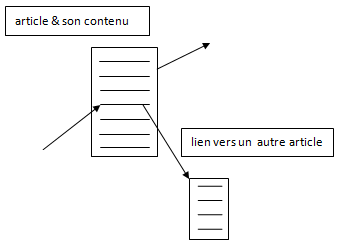
\includegraphics{images/23_image1.png}
\caption{Hypertexte -liens vers des articles}
\label{hypertexte}
\end{figure}

\textbf{Problème de cohérence}

\begin{itemize}
\item \underline{Web}: Cohérence \textit{"a posteriori"} 
						\vspace{0.1cm}
                       \\ Le web n'ayant pas d'organisation, on va devoir en trouver une : un index ou un moteur de recherche
      
\item \underline{Wikipedia}: Cohérence \textit{"a priori"}
							\vspace{0.1cm}
                             \\ Une structure existe déjà, définie par les rédacteurs, les modérateurs et les règles de structure.
\end{itemize}

Le succès du Web réside dans la possibilité de trouver une structure à ce dernier, notamment grâce à l'algorithme PageRank. Altavista, Google, Lycos, ... proposent tous leur version de moteur de recherche. C'est grâce à l'efficacité de PageRank que Google s'est imposé largement comme moteur de recherche dominant.

\subsection{Le Web est un graphe orienté}
\begin{itemize}
\item \underline{Chemin dans un graphe orienté}: A $- \rightarrow$ B
\vspace{0.1cm}
\\Séquence de nœuds qui commence avec A et termine avec B et où chaque paire consécutive correspond à un lien orienté.

\item \underline{Connectivité}: 
\vspace{0.1cm}
\\Un graphe orienté est connexe s'il existe un chemin orienté entre chaque paire de nœuds.
\end{itemize}

\subsection{Composant fortement connexe (CFC) \\ \textit{Strongly Connected Component (SCC)} }

À l'intérieur d'un graphe orienté, un composant fortement connexe est :
\begin{itemize}
    \item Un ensemble de nœuds tel qu'il existe un chemin orienté entre                   chaque paire.
    \item L'ensemble ne fait pas partie d'un plus grand environnement qui               à la même propriété. 
\end{itemize}

\begin{figure}[!ht]
\centering
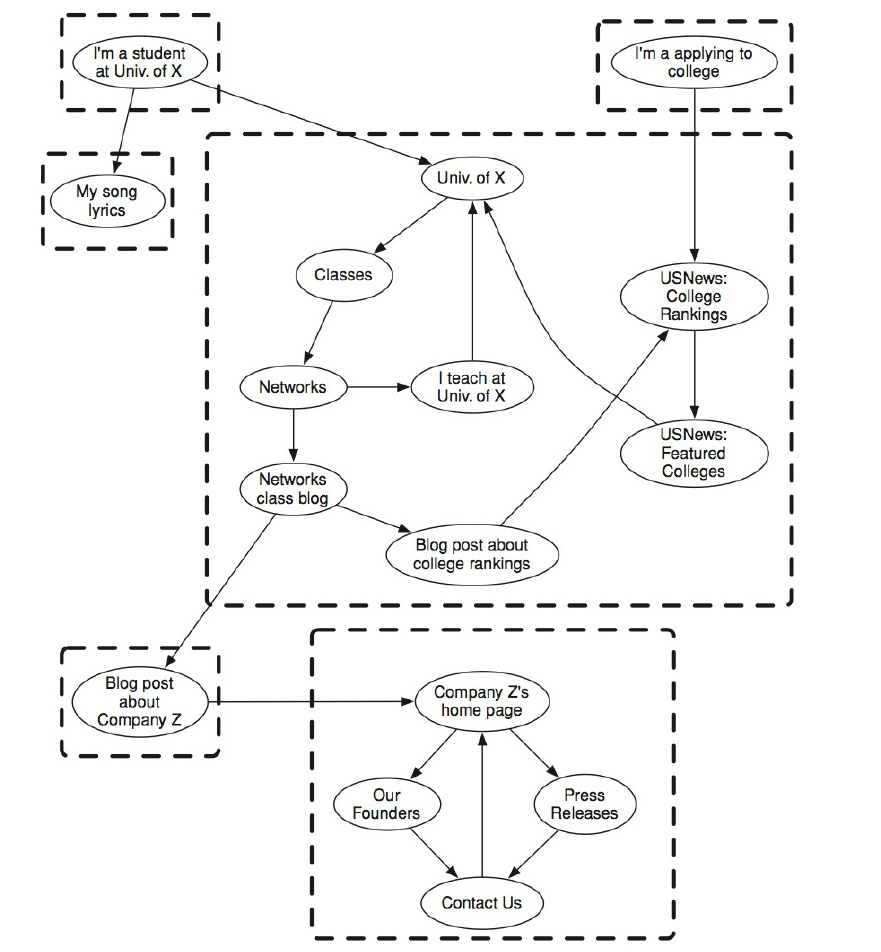
\includegraphics[scale=0.3]{images/23_fig13-6.png}
\caption{Un graphe dirigé avec ses CFCs identifiés}
\label{cfc_exemple}
\end{figure}

Les CFCs forment un genre de \textit{"super noeud"}. Pour la connectivité, on peut ignorer la structure interne des CFCs.

\vspace{0.3cm}

On peut donc transformer le graphe en un graphe réduit : le CFC devient un unique nœud. Pour trouver un chemin dans le graphe original, il suffit de trouver un chemin dans le graphe réduit.
Un exemple de transformation de ce type est illustré sur la figure \ref{cfc_transformation}.
\vspace{0.3cm}

\begin{figure}[!ht]
\centering
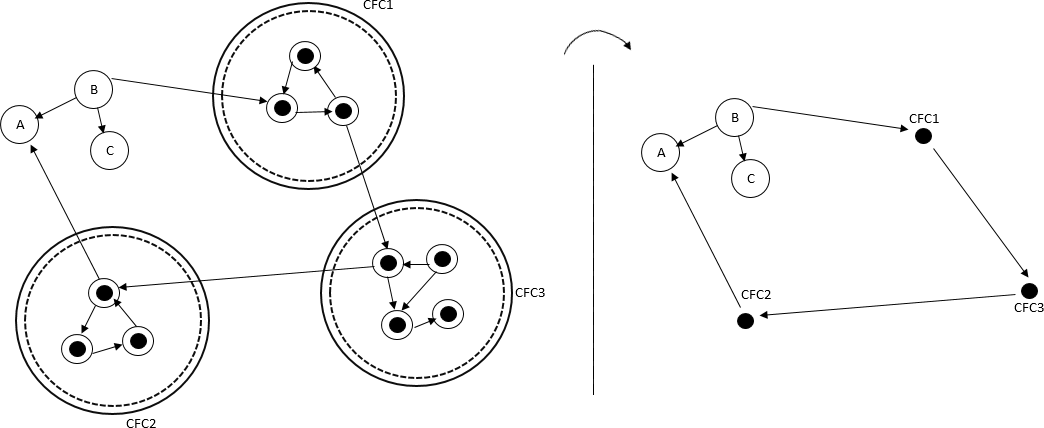
\includegraphics[width=0.85\linewidth]{images/23_schema2.png}
\caption{Exemple de transformation du graphe}
\label{cfc_transformation}
\end{figure}


\subsection{Nœud papillon (\textit{$\approx$ années 2000})}
	Maintenant, à quoi ressemble le graphe réduit du web ? Autour des années 2000, sa structure était proche de celle d'un nœud papillon, tel que celui représenté sur la figure \ref{noeud_papillon}.
	
	\begin{figure}[!ht]
		\centering
		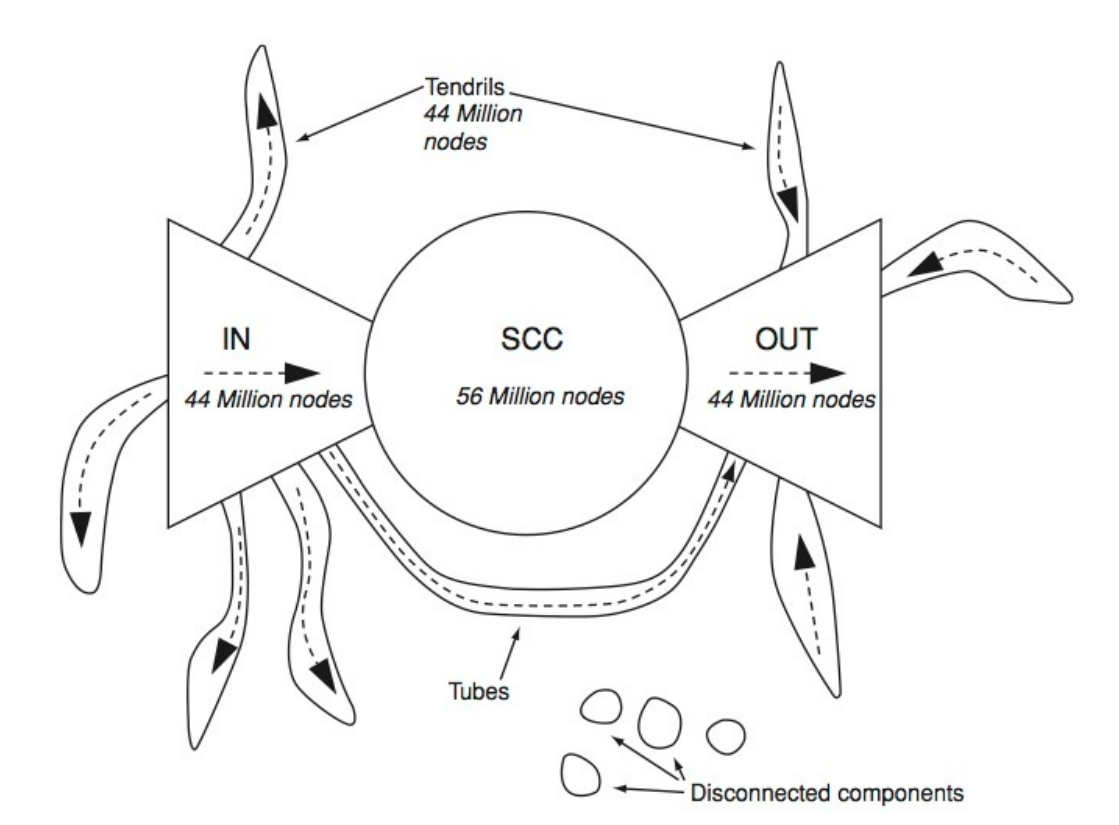
\includegraphics[scale=0.25]{images/23_fig13-7.png}
		\caption{Structure en nœud papillon du web}
		\label{noeud_papillon}
	\end{figure}
	
	On repère trois composants principaux :
	\begin{itemize}
	\item Un composant "in", qui contient des liens hypertextes sortants.
	\item Un composant fortement connecté principal, qui forme un "noyau".
	\item Un composant "out", qui contient beaucoup de liens hypertextes entrants.
	\end{itemize}


\subsection{Émergence du Web 2.0 (\textit{$\ge$ années 2000})}
L'émergence du Web 2.0 se déroule entre 2000 et 2010. Il s'agit en fait d'un changement d'attitude général des certains acteurs importants du web conduisant à une structuration de la toile basée sur trois grands principes. 
\begin{enumerate}
    \item \underline{Création collaborative} de contenu plutôt que des pages personnelles.
    \item \underline{Services} vers lesquels sont transférés les données personnelles. Au lieu de publier du contenu  sur des sites personnels, les gens se tournent vers des services pour publier leur contenu (par exemple Youtube, Flicker, Github...)
    \item \underline{Personnes} au lieu des documents. On n'identifie plus un document en fonction de son contenu, mais en fonction de son auteur ou de la personne qui en est le sujet.
\end{enumerate} 

\vspace{0.3cm}
%\begin{minipage}{15cm}
\textbf{Technologies utilisées:}
    \begin{itemize}
        \item Blogs (Skyblog), ensuite détrônés par les réseaux sociaux (Facebook, Twitter, MySpace, Friendster...)
        \item Deep Web : création de page à la demande (créer un nouveau profil, une page Wikipédia, un groupe d'intérêt...)
        \item Cloud : regroupement et partage de ressources "à la demande", permet plus d'élasticité (adaptation en fonction des besoins)
    \end{itemize}
%\end{minipage}

\vspace{0.5cm}       

\newpage

%\hline 
\vspace * {0.5cm}
    \fbox{\textbf{Un petit bout d'histoire}}
    
    \vspace{0.3cm}
    
    \underline{Quelques précurseurs} :
    
    \begin{itemize}
        \item \underline{1945 - Vannevar Bush} : Conseiller du président des États-Unis, Roosevelt\\ 
        Il a écrit un article intitulé "As We May Think" dans lequel il explique son appareil électronique relié à une bibliothèque et capable d'afficher des livres et de projeter des films appelé "Memex".
        \item \underline{1934 - Paul Otlet} : Documentaliste\\ 
        Il avait imaginé un système où l'on pourrait faire des recherches et consulter le résultat de ces recherches sur un écran. Cette intuition d'un pre-internet est à l'origine d'une structuration des ressources des bibliothèques. Il est aussi un pionnier des microfiches, des fiches indépendantes qui stockent des informations, ayant une ressemblance non-négligeable avec les pages web d'aujourd'hui.
        \item \underline{1990 - Tim Berners-Lee et  Robert Cailliau - CERN} : Inventeur du World Wide Web\\
        Ils se sont inspirés des ecrits de Vannevar Bush pour inventer le WWW, avec sa structure de pages indépendantes reliées par des liens hypertextes.
    \end{itemize}
    
\vspace * {0.5cm}   
%\hline 


\section{Recherche dans le Web} %chapitre 14
Comment trouver une information ?
\vspace{0.3cm}

\underline{1960} : Concept de mot-clé $\rightarrow$ Limitations fortes

\begin{itemize}
    \item Limitations dues au concept de mot
        \begin{itemize}
            \item Synonymie : plusieurs mots pour le même concept.
            \item Polysémie : un mot pour plusieurs concepts.\\
            Par exemple les noms propres peuvent référer à plusieurs personnes, des lieux et des organisations.

        \end{itemize}
        
        Autrement dit, il n'y a pas de bijection entre les mots et les concepts.
        
    \item Limitations dues à l'abondance d'informations.\\
    $\left. %\text{
    \parbox{0.5\linewidth}{
        \begin{itemize}
            \item \underline{Avant}: Les informations sur le web étaient rares. 
            \item \underline{Maintenant}: Il y a beaucoup trop d'informations.
        \end{itemize}
        %}
        } \hspace{0.5cm} \right 
        \}
        $ Plus grand problème du web
\end{itemize}
    
	Pour résoudre le problème de surabondance d'informations, il faut trouver une façon de savoir quelle page est la meilleure. Comment faire ce choix ?
	
	La meilleure solution est d'utiliser l'information contenue dans la structure du réseau.


%\end{document}



